\documentclass[%draft,
    a4paper,
    11pt, % use explicit paper size
    headinclude, footexclude,
    notitlepage,
    headsepline,
    pointlessnumbers,
    ]{scrartcl}
\usepackage{pslatex} % -- times instead of computer modern

\typearea{12}
\usepackage{scrpage2} % for headers
 \setkomafont{pagehead}{\scshape\small}
 \setkomafont{pagenumber}{\scshape\small}
 \ihead[]{Martin Schoeberl}
 \ohead[]{CV}

% \ofoot[]{} \cfoot[]{} \ifoot[]{}

\usepackage{hyperref}
\usepackage{booktabs}
\usepackage{graphicx}
\usepackage{amsmath}
\usepackage{dcolumn}
\newcommand{\cc}[1]{\multicolumn{1}{c}{#1}}
\newcolumntype{d}[1]{D{.}{.}{#1}}
\usepackage{boxedminipage}

\newcommand{\excelwidth}{\columnwidth}

\newcommand{\code}[1]{{\textsf{#1}}}


\begin{document}

\pagestyle{scrheadings}


%\begin{center}
%\vspace{3cm}
%{\usekomafont{title}\huge Curriculum Vitae}\\
%\bigskip
%\bigskip
%\end{center}

%\section{Short CV}
%
%Martin Schoeberl is associate professor at the Technical University of Denmark, at
%the Department of Applied Mathematics and Computer Science. He completed his
%PhD at the Vienna University of Technology in 2005 and received the Habilitation
%in 2010. Martin Schoeberl's research focus is on time-predictable computer architectures
%and on Java for hard real-time systems. During his PhD studies he developed the
%time-predictable Java processor JOP, which is now in use in academia and in
%industrial projects. His research on time-predictable computer architectures is
%currently embedded in the EC funded project T-CREST.

%\section*{Letter of Application (Ref: 00000771)}
%\medskip
%December 31, 2019\\
%\\
%University of Freiburg\\
%Faculty of Engineering\\
%Dean\\
%Georges-Koehler-Allee 101\\
%79110 Freiburg, Germany\\
%\\
%\medskip
%\\
%Dear Dean,
%\medskip
%\\
%herewith I apply for the position of a Full Professorship for Computer Architecture.
%Currently I am associate professor at the Technical University of Denmark (DTU), at
%DTU Compute with a tenured position.
%
%I have enclosed my Curriculum Vitae, research and teaching plan and 
%the list of publications. I am at your service, if you need
%further information, and look forward to hear from you.
%\medskip\\
%Sincerely,\\
%\medskip\\
%Martin Schoeberl
%Straussengasse 2-10/2/55\\
%A-1050 Vienna\\
%Austria\\
%\url{mailto:mschoebe@mail.tuwien.ac.at}\\
%Tel. +43 1 58801 18207
%\textbf{Don't forget personal details form!}

\newpage

\section*{Curriculum Vitae}


\begin{tabular*}{0.7\textwidth}[h!]{@{\extracolsep{\fill} } l r}
\parbox[b]{11 cm}{Assoc. Prof. DI Dr.~Martin Schoeberl\\
Mariendalsvej 25, 1\\
2000 Frederiksberg\\
Denmark\\
\url{mailto:masca@dtu.dk}\\
\url{http://www.imm.dtu.dk/~masca/}} &
% \includegraphics[width=0.4\textwidth]{figures/distributed}\\
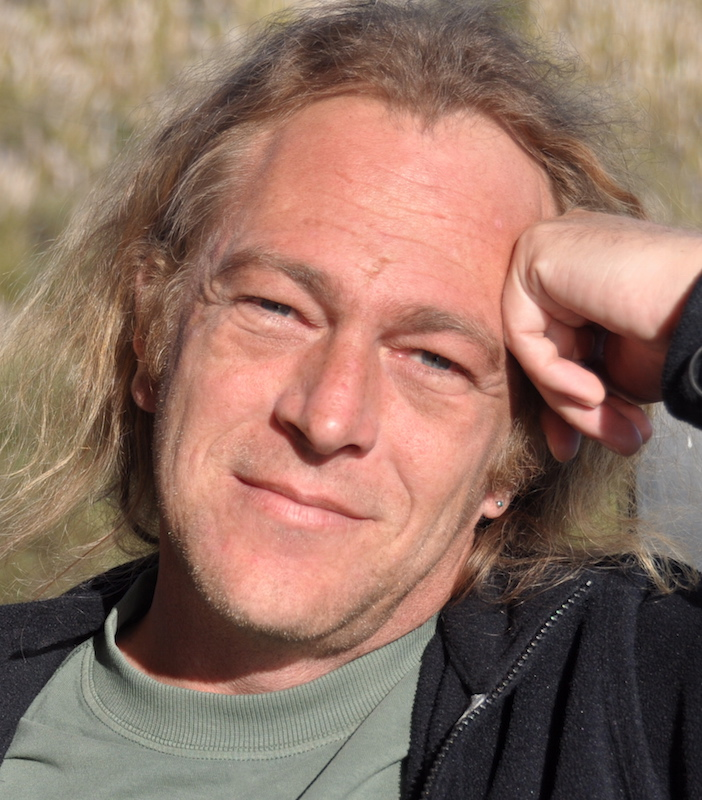
\includegraphics[width=3cm]{martin_small}\\
\end{tabular*}

\subsection*{Education}

\begin{tabular}{rl}
December 2010 & Habilitation at TU Vienna \\
April 2005   & PhD Degree in Computer Engineering\\
             & with distinction from TU Vienna, date: 11.4.2005\\
2000 -- 2004 & PhD Studies of Computer Engineering at the TU Vienna\\
\\
June 2000    & Conservatory Diploma in Jazz guitar at the\\
             & Gustav Mahler Conservatory, Vienna\\
Summer 1999  & Studies of Jazz guitar at the\\
             & Berklee College of Music, Boston, USA\\
\\
November 1994 & Master's Degree in Computer Science from TU Vienna\\
\\
1993 -- 2000 & Studies of Jazz guitar at the\\
             & Prayner and Gustav Mahler Conservatory, Vienna\\
\\
1986 -- 1994 & Studies in Computer Science at the TU Vienna\\
May 1986 & School leaving examination, with distinction\\
1980 -- 1986 & Engineering School for Communications Engineering\\
             & and Electronics in St.\ P\"olten\\
\end{tabular}

\subsection*{Employment}
\begin{tabular}{rl}
Since 2010    & Associate Professor at the Department of Applied Mathematics and\\
             & Computer Science, Technical University of Denmark\\
2005 -- 2009 & Assistant Professor at the Institute of Computer Engineering, TU Vienna\\
\\
1996         & Civilian Service in Vienna\\
Since 1994   & Self-employed with projects in automation and supervision for\\
             & the Lower Austrian energy provider (EVN), Balfour Beatty,\\
             & and the Austrian railway company (\"OBB)\\
\\
1992 -- 1994 & Software engineer at Wirtschafts- und Sozialwissenschaftliches Rechenzentrum\\
1987 -- 1991 & Software engineer at COIN Computerentwicklungen GmbH\\
1986 -- 1987 & Software engineer at SYSGRAPH Computergraphik GmbH\\
\end{tabular}

\clearpage

%\section{Curriculum Vitae}

Currently I am associate professor at the Technical University of Denmark (DTU), at
DTU Compute with a tenured position.
%I have applied for promotion to a full professor at DTU Compute.
From 2005 to 2010 I was assistant professor at the Institute of Computer Engineering, Vienna
University of Technology.
I completed my PhD at the Vienna University of Technology in 2005 and
received the Habilitation in Computer engineering in 2010.

% turned in the Habilitation in 2009.
%Habil awarded 21.12.2010.

My research focus is on time-predictable computer architectures,
multi-core system-on-chip for real-time systems, and
on Java for hard real-time systems. During my PhD, I developed the
time-predictable Java processor JOP. This processor is currently
being used in industrial projects and is the basis for further
research on chip-multiprocessors for real-time systems. The Java
processor is not only open-source, it is also being used at other
universities as a basis for real-time Java research, and, in
addition, is the subject of an active online community (i.e., a
mailing list with 716 members). JOP is the only Java processor for
which the execution time can be easily analyzed and a worst-case
execution time (WCET) analysis tool is available.

The result of my PhD thesis, the real-time Java processor JOP,
enabled my participation in the EU project JEOPARD (Java Environment
for Parallel Realtime
Development).\footnote{\url{http://www.jeopard.org/}} The JEOPARD
project started in January 2008 and the overall project budget is EUR
3.2 million.
%Led by the Open Group, the JEOPARD consortium includes
%four universities and research institutes: The University of York,
%the TU Vienna, FZI and the Technical University of Cluj-Napoca; three
%industrial manufacturers: EADS, RadioLabs and SkySoft; and two
%embedded systems technology suppliers: aicas and Sysgo.
I was responsible for the Austrian part of the proposal, representing the
TU Vienna in the project, and I lead the ``Architecture"
work-package in JEOPARD.

My work on time-predictable architectures led to the \textbf{EC funded project
T-CREST} (Time-predictable Multi-Core Architecture for Embedded
Systems).\footnote{\url{http://www.t-crest.org/}}
T-CREST started September 2011 and the overall project budget
is EUR 3.8 million. \textbf{I led the funding proposal and was technical lead of
T-CREST.}

Furthermore, my expertise in real-time Java and the implementation of
the time-predictable JOP led to my membership of the Expert Group for
the standard on Safety Critical Java (JSR
302).\footnote{\url{http://jcp.org/en/jsr/detail?id=302}}
%which is managed by the Java Community Process and led by Doug Locke.

%According to Microsoft Academic Search I am \textbf{ranked on place 5 for the Top authors in Real-Time \& Embedded Systems} in the last 5 years.\footnote{Last accessed on 13.8.2015:
%\url{http://academic.research.microsoft.com/RankList?entitytype=2&topdomainid=2&subdomainid=19&last=5}}

% 2 on 28.1.2014
% position 5 on 18.1.2011
% 8 on 13.2.2012 (37 pubs, h 8)
% 4 on 4.6.2013 (33 pubs, field rating 7)

\subsection*{Industrial Experience}

Since 1986, I have been working in the area of computer engineering
and in the automation industry on distributed soft real-time systems.
Since 1994, I have been self-employed and occupied on projects in
embedded systems for automation and supervision. Four of the projects
were based on the Java processor JOP:\footnote{Three of the projects
are described in an invited paper for the IFAC 2008, available at
\url{http://www.jopdesign.com/doc/jop_app.pdf}} (1) A distributed
motor control system for Balfour Beatty; (2) An industrial lift
controller (Ankara, Turkey); (3) A remote control system for the
Lower Austrian energy provider EVN; and (4) A railway control support
system for single track lines for the Austrian railway company \"OBB.
All those systems are embedded systems where I designed the hardware
with an FPGA, for three of the four, the external hardware (electronics),
and wrote the embedded software. I consider all those tasks at the center
of applied computer engineering.
Those projects are all embedded real-time systems, systems that
interact with the physical world, i.e., cyber physical systems.

Moreover, I have supported the Austrian SME DECOMSYS in the chip
design for the real-time communication controller for the FlexRAY bus
during a half year project.
I designed the bus frontend with the synchronization unit and the
interface to the PowerPC.

%\subsubsection*{A Cyber Physical System}
%
%The last system I developed in my self employed time, the railway control, is
%a good example of a medium complex cyber physical system.
%The controllers are embedded in the physical system of a locomotives.
%They need to be aware about the environment, i.e., they
%know their GPS based position and the layout of the track and individual
%track segments, as defined by physical railway entities. The controller
%communicates with the locomotive driver and with the central station
%for command and control. Several controllers are active at any time
%and therefore form a distributed system. Furthermore, the whole system
%has to work under real-time constraints: there was a maximum time between
%detecting a dangerous situation and alarming the driver and the supervisor
%in the central station.
%
%For this system I developed the hardware and the software of the controller
%and designed the network protocol to interact with the central station.
%I consider this relatively complex, \textbf{industrial cyber physical system a good background for
%the position of a Professor of Cyber-Physical and Embedded Systems.}

\subsubsection*{Benefit for Academia}

My extended experience in research and development for industry
provides a good background for research in the area of 
embedded real-time systems and
cyber-physical systems.
%computer engineering.
I returned to academia due to personal interest
and to solve some of the fundamental problems I had seen during my
industrial work. Finally, my industrial experience and leading
development projects provides profound knowledge to establish and
lead an independent research group.


\subsection*{Summary of Scientific Work}

\begin{itemize}
  \item 27 journal articles
  \item 150 original, peer reviewed conference and workshop
      publications
  \item 4 books
  \item 1 patent
  \item 4176 citations, h-index of 36
  \item several invited talks % 16 invited talks
  \item Reviewer for several journals and PC member of several
      conferences
  \item Member of the Expert Group for the Safety Critical Java
      Specification
\end{itemize}

%\subsection*{References}
%
%\begin{itemize}
%  \item Edward Lee, University of California, Berkeley, \url{mailto:eal@berkeley.edu}
%  \item Andy Wellings, University of York, UK, \url{mailto:andy@cs.york.ac.uk}
%  \item Jens Spars{\o}, Technical University of Denmark, \url{mailto:jspa@dtu.dk}
%\end{itemize}

\subsection*{Research Visits}

\begin{itemize}
  \item Fall 2019, University of California, Berkeley
  \item Winter 2018/19, University of California, Berkeley
  \item Winter 2015/16, University of California, Berkeley
  \item Winter 2012/13, University of California, Berkeley
  \item Fall 2009, University of California, Berkeley
  \item April 2008, Aalborg University, Denmark
  \item August 2007, Aalborg University, Denmark
  \item February (+ spring part time) 2006, CBS, Copenhagen,
      Denmark
\end{itemize}

\subsection*{Funding}

\begin{itemize}

\item 2016--2021: Time-predictable Control Systems (PREDICT),
Danish Council for Independent Research | Technology and Production
  Sciences under contract 6111-00363; DKK 5,170,177.-
  
  \item 2013--2016: Hard Real-Time Embedded Multiprocessor Platform - RTEMP
  (Co-applicant, PI is Jens Spars{\o}), 
  Danish Research Council for Technology and Production
  Sciences under contract 12-127600; DKK 4,977,862.-
  
  \item 2012--2016: ICT COST Action IC1202 Timing Analysis on Code-Level (TACLe),
  Co-applicant and work package 2 lead.
  
  \item 2011--2014: FP7 EC project T-CREST (Time-predictable
  Multi-Core Architecture for Embedded Systems) under grant
  agreement number 288008; EUR 3,807,000.- (total), EUR 703,000.- for DTU.
  I \textbf{led the funding proposal} and was \textbf{technical coordinator of T-CREST}.
  The proposal was \textbf{ranked at position 4 out of 59} submissions.
  
  \item 2011--2014: Certifiable Java for Embedded Systems (\emph{Principal Investigator} and funding applicant),
   Danish Research Council for Technology and Production
   Sciences under contract 10-083159; DKK 5,058,000.-.
   
  \item 2008--2010: FP7 EC project JEOPARD (Java Environment for
      Parallel Realtime Development) under grant agreement number
      216682; EUR 3,170,000.- (total), EUR 167,000.- for the TU
      Vienna. I wrote the proposal part for TU Vienna and I am
      lead the work package on architectures. JEOPARD
      deals with the issues for chip-multiprocessor solutions for
      real-time Java.
      
  \item 2004--2007: \emph{Principal Investigator} and funding
      applicant (self employed) for the national SME funding
      project: Implementation of the CLDC standard for real-time
      systems on a Java processor, EUR 80,000.-
      
\end{itemize}

\subsection*{Invited Talks and Tutorials}

\begin{itemize}
\item  September 20, 2020, ``Software-Defined Hardware: Digital Design with Chisel'', one day tutorial at ESWEEK, on-line
\item September 18, 2020, ``Digital Design in Chisel'', RISC-V Day Vietnam 2020
\item  September 4, 2020, ``Software-Defined Hardware: Digital Design with Chisel'', one day tutorial at FPL, on-line
\item January 29, 2020, ``Is Chisel Ready for Class?'',
Chisel Community Conference, Western Digital, Milpitas, CA
\item October 13, 2019, ``Hardware Design in the 21st Century with the Object Oriented and Functional Language Chisel'', one day tutorial at ESWEEK, New York, USA
\item September 13, 2019, ``Hardware Design in the 21st Century with the Object Oriented and Functional Language Chisel'', one day tutorial at FPL, Barcelona, Spain
\item February 11, 2019, ``A Time-predictable Multicore Processor Architecture for Real-Time Systems'', DREAM seminar, University of California, Berkeley, EECS
\item November 13, 2018, ``Fast Prototyping for Computer Architecture Research with Chisel'',
Chisel Community Conference, University of California, Berkeley, CA
\item August 30, 2018, ``Hardware Design in the 21st Century with the Object Oriented and Functional Language Chisel'', one day tutorial at FPL, Dublin, Ireland
\item June 11, 2018, ``Time-predictable Computer Architecture with Time Division Multiplexing'',
Optimizing Real-Time Systems Working Group Meeting, Paris, France
 \item November 3, 2016, ``T-CREST: Time-predictable Multi-Core Architecture for Embedded Systems'',
      Dagstuhl seminar, Dagstuhl, Germany
\item June 15-16, 2016, ``Chisel Tutorial'', University of Augsburg, Germany.
\item June 14, 2016, ``T-CREST: Time-predictable Multi-Core Architecture for Embedded Systems'',
University of Augsburg, Germany
%\item several missing, e.g., Augsburg
 \item November 16, 2012, ``T-CREST: Time-predictable Multi-Core Architecture for Embedded Systems'',
      DREAM seminar, University of California, Berkeley, EECS
  \item July 6, 2011, ``A Time-predictable Microprocessor: the Patmos Approach'',
      11th International Forum on Embedded MPSoC and Multicore (MPSoC), 2011, Beaune, France
  \item September 19--23, 2010, ``The Java Optimized Processor: Java in a Field-Programmable Gate Array",
      JavaOne, San Francisco, California, USA
  \item June 29, 2010, ``Schedule Memory Access, not Threads",
      10th International Forum on Embedded MPSoC and Multicore (MPSoC), 2010, Gifu city, Gifu, Japan
  \item May 7, 2010, ``Real time JAVA in FPGA based systems",
      Prevas 25 year celebration, Copenhagen, Denmark
  \item December 10, 2009, ``A Java Processor in an FPGA for
      Real-Time Systems", Sun Labs, Menlo Park CA, USA
  \item March 5, 2009, ``JOP, a Java Processor for Embedded
      Real-time Systems", University of Lugano, Switzerland
  \item February 3, 2009, ``JEOPARD, Multi-Core and Safety
      Critical Java", The Open Group, Real-Time Embedded Systems
      Forum, San Diego, California
  \item September 24, 2008, JTRES 2008 Panel: Approaches to
      Multi-Core Processing
  \item April 2008, Aalborg University, Denmark
  \item February 2008, University of Augsburg, Germany
  \item September 2006, University College Vitus Bering, Denmark
  \item September 2006, Workshop on Java in Embedded Systems,
      CISS, ITU Copenhagen
  \item June 2006,  Dept. of Informatics, CBS, Copenhagen
  \item March 2006, Workshop on Java in Embedded Systems, CISS,
      Aalborg
  \item August 2004, Dept. of Computer Science, Lund Institute of
      Technology, Sweden

\end{itemize}

\subsection*{Community Services}

\begin{itemize}
  \item General chair ARCS 2019 in Copenhagen
  \item EU projects track chair DATE 2019
  \item Program chair JTRES 2009, 2016
  \item Program chair WCET 2016
  \item Program Co-Chair ISORC 2015
  \item Workshop chair JTRES 2012 in Copenhagen
  \item Track Co-Chair ACM SAC 2011
  \item Editorial Board Member of Journal of Systems Architecture (JSA)
  \item Associate editor: EURASIP JES, IJERTCS
  \item Guest editor for the special issue on \emph{Java
      Technologies for Real-Time Distributed and Embedded
      Systems} in Concurrency and Computation: Practice and
      Experience
  \item Workshop chair JTRES 2007 in Vienna
  \item Expert Group member of the Safety Critical Java
      Technology Specification (JSR 302)
  \item PC member JTRES 2006--2016
  \item PC member FPL 2007--2015
  \item PC member ACM SAC 2010--2021
  \item PC member ISORC 2010, 2012--2020
  \item PC member RTNS 2012, 2017
  \item PC member WCET 2012, 2015--2019
  \item PC member SIES 2016--2018
  \item PC member SEUS 2010, 2013--2016
  \item PC member Transact 2010
  \item PC member PPPJ 2013, 2014, ECRTS WiP 2013
  \item PC member SSV 2014
  \item PC member HiRES 2014--2016
  \item PC member Ada-Europe 2016
  \item PC member RTSS 2018
  \item PC member RTAS 2019
  \item PC member DESTION 2019, 2020
  \item Reviewer for embedded systems journals: RTS, JSA, EURASIP JES,
      TECS, TCAD, TII, TPDS, TCAS, SP\&E, IET Software, TPDS, S P\&E, IJERTCS, ESL, TAES,...
%  \item Secondary reviewer for: RTSS, ECRTS, DATE, FPL, CPS
\end{itemize}

\subsection*{Teaching}

\begin{itemize}
  \item Verification of Digital Designs (2020)
  \item Computer Architecture and Engineering (since 2010)
  \item Advanced Computer Architecture (since 2011)
  \item Digital Electronics (since 2011)
  \item Computer Architecture VO (2006--2008)
  \item Computer Architecture Lab (2006--2008)
  \item The Java Virtual Machine in Hardware VL (2005--2009)
  \item Very Small Information Systems (2006 at CBS, Copenhagen)
  \item Distributed Systems (2006 at CBS, Copenhagen)
  \item Electrical Engineering Lab (2005--2006)
  \item Digital Signal Processor Lab (2005--2008)
  \item Bachelor Project and Seminar (since 2006)
\end{itemize}

\subsection*{Supervised Theses}

\subsubsection*{Guiding PostDocs}

\begin{itemize}
  \item Torur Biskopsto Strom
  \item Wolfgang Puffitsch
  \item Florian Brandner
\end{itemize}


\subsubsection*{PhD Theses}

\begin{itemize}
\item Eleftherios Kyriakakis, FORA Open Source Fog Node: Hardware support for virtualization, current
\item Torur Biskopsto Strom, Real-Time Multi-Core Communication and Synchronization, 2019
%\item Oktay Baris, Communication in Real-Time Multicore Systems, current
  \item Luca Pezzarossa, Dynamic Partial Reconfiguration in FPGA based Multi-core Real-time Embedded Systems, 2018 (Co-supervision)
  \item Rasmus Bo S{\o}rensen, Hardware/Software tradeoffs in Real-Time Multiprocessor Platforms, 2016 (Co-supervision)
  \item Sahar Abbaspourseyedi, Time-predictable VLIW Processor, 2015
  \item Evangelia Kasapaki, Asynchronous Network-on-Chip for Time-Predictable
     Multi-Core Embedded Systems, 2015 (Co-supervision)
  \item Juan Rios, Certifiable Java for Embedded Systems, 2014
  \item Alexander Jordan, Restricted Global Scheduling and Cache Optimization Techniques for VLIW Architectures, (Co-supervision with TU Vienna), 2014
  \item Wolfgang Puffitsch, Real-Time Garbage Collection for
      Multiprocessor Systems, 2012
  \item Christof Pitter, Time-Predictable {Java}
      Chip-Multiprocessor, 2009  (Co-supervision)
\end{itemize}

\subsubsection*{Master Theses}

\begin{itemize}

\item Emad Jacob Maroun, Instruction Scheduler for the Dual-Issue Patmos Pipeline, 2019
\item Roman Birca, SystemC Tracing for Observability and Profiling, 2018
\item Daniel Sanz Ausin, Audio Processing on a Multicore Platform, 2017
\item Philipp Degasperi, Method Cache for Patmos, 2014
\item Marco Ziccardi, A Time-Composable Operating System for the Patmos Processor, 2014
\item David~VH Chong, Memory Access Arbitration for the Patmos Chip-Multicore Processor, 2014
\item Edgar Lakis, FPGA implementation of time predictable memory controller for a chip-multiprocessor system, 2013
  % TUV TP memo controller
  \item T\'{o}rur Biskopst\o{} Str\o{}m, Safety-Critical Java 3D Desktop Printer, 2013
  \item Rasmus Bo S{\o}rensen, Programming of the T-CREST real-time multi-processor platform, 2012
  \item Stefan Hepp, Worst-Case Execution Time Driven Method Inlining for Embedded Java Processors, 2011
  \item Thomas Bowley, Migrating a backbone network product platform for a wireless sensor system, from assembler/C to a higher level embedded Java paradigm, 2010
  \item Peter Hilber, Hardware Transactional Memory for a
      Real-Time Chip Multiprocessor, 2010
  \item Benedikt Huber, Worst-Case Execution Time Analysis for
      Real-Time {Java}, 2009
  \item Christian Stoif, Implementation and Performance of
      Synchronization Methods for Dual-Core Engine
      Control-Systems, 2008
  \item Wolfgang Puffitsch, {picoJava-II} in an {FPGA}, 2007
  \item Mikael Lundsgaard and Jens Kritian Rasmussen, JOPSPEECH,
      Embedded Java Speech Recognition SDK, 2007, CBS Copenhagen
  \item Kasper Hansen, Bluetooth API for JOP, 2007, CBS
      Copenhagen
\end{itemize}

%\subsubsection*{Bachelor}


\subsection*{Links}

\begin{itemize}
  \item Personal page at DTU:
      \url{http://www.imm.dtu.dk/~masca/}
  \item Google Scholar profile:
\url{http://scholar.google.com/citations?user=wiRNmwUAAAAJ&hl=en&oi=ao}
%  \item Personal page at TU Vienna:
%      \url{http://ti.tuwien.ac.at/rts/people/schoeberl}
  \item GitHub page: \url{https://github.com/schoeberl}
  \item PhD thesis:
      \url{http://www.jopdesign.com/thesis/thesis.pdf}
%Publication list:
%     \url{http://scholar.google.com/scholar?q=+''martin+schoeberl''+author:m-schoeberl}
  \item JOP web site: \url{http://www.jopdesign.com/}
%  \item JOP Wiki: \url{http://www.jopwiki.com/}
%  \item JOP mailing list:
%      \url{http://groups.yahoo.com/group/java-processor/}
\end{itemize}


%Collaborations:
%
%Thomas Henties, Siemens AG; James J. Hunt, aicas; Doug Locke, Locke
%Consulting, LLC; Kelvin Nilsen, Aonix NA, Andy Wellings, University
%of York; Florian Brandner, Vienna University of Technology; Tommy
%Thorn, Unaffiliated Researcher; Walter Binder, University of Lugano;
%Alex Villazon, University of Lugano; Philippe Moret, University of
%Lugano; Wolfgang Puffitsch, Vienna University of Technology; Peter
%Puschner, Vienna University of Technology; Stephan Korsholm, Aalborg
%University; Anders P. Ravn, Aalborg University; Tomas Kalibera,
%Purdue University; Trevor Harmon, University of California, Irvine;
%Raimund Kirner, Vienna University of Technology; Christian Thalinger,
%Vienna University of Technology; Jan Vitek, Purdue University;
%Christof Pitter, Vienna University of Technology; Hans Sondergaard,
%Aalborg University; Bent Thomsen, Aalborg University; Rasmus
%Pedersen, CBS Copenhagen; Flavius Gruian, Lund University; Per
%Andersson, Lund University; Krzysztof Kuchcinski, Lund University

%Add:
%	Master thesis
%	PhD thesis
%	add invited talk topics

%Master based on JOP:
%
%The students where Jan Egberg Lauritzen and Mads Pedersen - they
%finalized their master of science thesis in december 2005.
%Unfortunately their thesis is written in dansish, but I send you the
%abstract.
%
%Best regards Finn
%
%Abstract English title: Evaluation of Java for developing embedded
%real-time systems using an existing "Java Optimized Proccesor" In
%this Master Thesis, the usage of Java for developing embedded
%real-time systems is evaluated based on a "Java Optimized Processor"
%platform (JOP). The processor is an implementation of a JVM in an
%FPGA. The evaluation shows that Java is suitable for real-time
%critical applications using JOP as the platform, because executing a
%Java program is deterministic on this platform. A proprietary
%real-time profile developed for JOP and inspired by Ravenscar-Java
%has been described. Real-time applications can be optimized by moving
%time critical program parts closer to hardware by using the
%flexibility in JOP as it is based on a FPGA platform. In the Master
%Thesis, an example of this hardware/software co-design is made. A
%noticeable optimization measured in clock cycles used in the
%processing is achieved. For examining development with JOP, a
%frequency counter as an example of a hardware close real-time system
%has been successfully implemented. Key words: Embedded real-time
%systems, Java, RTSJ, Ravenscar-Java, Java Optimized Processor, JOP,
%FPGA, VHDL, HW/SW co-design.



\end{document}
